\documentclass[11pt]{article}
\usepackage[a4paper,margin=29mm]{geometry}
\usepackage[T1]{fontenc}
\usepackage{lmodern}
\usepackage{microtype}
\usepackage{mathtools,amssymb,amsthm}
\usepackage{enumitem}
\usepackage{needspace}
\usepackage{xcolor}
\usepackage{tikz}
\definecolor{linkblue}{RGB}{25,65,110}
\usepackage[colorlinks=true,linkcolor=linkblue,citecolor=linkblue,urlcolor=linkblue]{hyperref}
\usepackage[nameinlink,capitalise,noabbrev]{cleveref}
\hypersetup{
  pdftitle={Radius of comparison equals half the mean dimension},
  pdfsubject={The integer-action case of the Phillips-Toms conjecture},
  pdfauthor={OpenAI},
  pdfkeywords={radius of comparison, mean dimension, minimal dynamics, small boundary property, Jiang-Su stability, nuclear dimension, complex cobordism, nilpotence}
}
\pdfgentounicode=1
\pdfinfoomitdate=1
\pdftrailerid{}
\pdfsuppressptexinfo=15
\newtheorem{theorem}{Theorem}[section]
\newtheorem{proposition}[theorem]{Proposition}
\newtheorem{lemma}[theorem]{Lemma}
\newtheorem{corollary}[theorem]{Corollary}
\theoremstyle{definition}
\newtheorem{definition}[theorem]{Definition}
\newtheorem{notation}[theorem]{Notation}
\theoremstyle{remark}
\newtheorem{remark}[theorem]{Remark}
\AddToHook{env/lemma/begin}{\crefalias{theorem}{lemma}}
\AddToHook{env/proposition/begin}{\crefalias{theorem}{proposition}}
\AddToHook{env/corollary/begin}{\crefalias{theorem}{corollary}}
\numberwithin{equation}{section}
\newcommand{\Z}{\mathbb Z}
\newcommand{\R}{\mathbb R}
\newcommand{\C}{\mathbb C}
\newcommand{\N}{\mathbb N}
\newcommand{\T}{\mathbb T}
\newcommand{\Sph}{\mathbb S}
\DeclareMathOperator{\rc}{rc}
\DeclareMathOperator{\mdim}{mdim}
\DeclareMathOperator{\supp}{supp}
\DeclareMathOperator{\rank}{rank}
\DeclareMathOperator{\id}{id}
\DeclareMathOperator{\cofib}{cofib}
\DeclareMathOperator{\fib}{fib}
\DeclareMathOperator*{\hocolim}{hocolim}
\DeclareMathOperator*{\holim}{holim}
\setlist[enumerate]{label=\textup{(\roman*)},leftmargin=*}
\setlist[itemize]{leftmargin=*}
\setlength{\emergencystretch}{1.5em}
\allowdisplaybreaks[1]

\title{Radius of comparison equals\\half the mean dimension}
\author{OpenAI}
\date{September 25, 2026}

\begin{document}
\maketitle
\begin{abstract}
We prove the integer-action case of the Phillips--Toms conjecture:
for every minimal homeomorphism of an infinite compact metrizable space,
the radius of comparison of its crossed product equals one half of its
mean dimension, including equality at infinity. For these systems, zero
mean dimension and the small boundary property are equivalent to
Jiang--Su stability and to finite nuclear dimension of the crossed
product; in this case its nuclear dimension is at most one.
\end{abstract}

\section{Introduction}
\label{sec:introduction}

Mean dimension measures the dimension needed per orbit coordinate.
Introduced by Gromov and developed by Lindenstrauss and Weiss, it remains
informative for compact dynamical systems whose ordinary covering
dimension is infinite \cite{Gromov1999,LindenstraussWeiss2000}.
Toms introduced the radius of comparison to measure the tracial gap
needed for comparison of positive elements of a C*-algebra
\cite[Definition~6.1]{Toms2006}. The Phillips--Toms conjecture relates
these dynamical and operator-algebraic quantities. We prove its
integer-action case, with the factor one half suggested by the relation
between complex vector-bundle rank and real dimension.

\subsection{The statement and conventions}

For a finite open cover \(\mathcal V\) of a compact space, let
\(D(\mathcal V)\) be the least order of a finite open refinement, where
the order is one less than the largest number of members with a nonempty
common intersection. For a homeomorphism \(h:X\to X\), put
\[
\mathcal U^{[a,b)}=\bigvee_{j=a}^{b-1}h^{-j}\mathcal U,
\qquad
\mdim(X,h)=\sup_{\mathcal U}
\lim_{N\to\infty}\frac{D(\mathcal U^{[0,N)})}{N}.
\]
The supremum ranges over finite open covers. The limit for each cover
exists by subadditivity and is finite; the supremum may be infinite.

We use the tracial formulation of the radius of comparison for nuclear
C*-algebras \cite[Definition~2.10]{Niu2024}; in this setting quasitraces
are traces. Let \(A\) be a unital nuclear C*-algebra with tracial states. Write
\(M_\infty(A)=\bigcup_{q\ge1}M_q(A)\), using the upper-left corner
inclusions. For positive elements \(a,b\in M_\infty(A)\),
\(a\precsim b\) denotes Cuntz subequivalence: there are matrices
\(x_j\), after passage to compatible finite corners, such that
\(x_j^*bx_j\to a\) in norm. For a normalized tracial state \(\tau\), set
\[
d_\tau(a)=\lim_{m\to\infty}(\tau\otimes\operatorname{Tr})(a^{1/m}),
\]
where \(\operatorname{Tr}\) is the unnormalized matrix trace.
We say that a finite \(r\ge0\) is a \emph{comparison bound} for \(A\) if
\begin{equation}
\label{eq:comparison-bound}
\bigl(d_\tau(a)+r<d_\tau(b)\ \text{for every normalized trace }\tau\bigr)
\quad\Longrightarrow\quad a\precsim b
\end{equation}
for all such positive elements. The radius of comparison \(\rc(A)\)
is the infimum of the comparison bounds, with \(\inf\varnothing=\infty\).

\begin{theorem}
\label{thm:main}
Let \(h\) be a minimal homeomorphism of an infinite compact metrizable
space \(X\). Then
\begin{equation}
\label{eq:main}
\rc\bigl(C(X)\rtimes_h\Z\bigr)=\frac12\mdim(X,h)
\qquad\text{in }[0,\infty].
\end{equation}
\end{theorem}

Infinitude and minimality imply that the action is free: a periodic orbit
would be a finite closed invariant subset equal to \(X\).
The crossed product is nuclear \cite[Section~3]{ElliottNiu2017} and
has tracial states, obtained from invariant probability measures and
the canonical conditional expectation.
Thus the conventions above apply. In particular, \Cref{thm:main}
asserts that infinite mean dimension forces infinite radius of
comparison, as well as identifying the exact constant at finite
positive mean dimension.

\subsection{Prior results and the remaining lower bound}

The two invariants arose in different settings. Toms's radius of
comparison records the dimension-to-rank obstruction to comparing
positive elements, extending the role of vector-bundle obstructions
in C*-algebra classification \cite[Section~6]{Toms2006}.
Giol--Kerr brought this obstruction into dynamics: they constructed
minimal systems of positive mean dimension whose crossed products have
arbitrarily large radii of comparison
\cite[Section~2 and Theorem~2.2]{GiolKerr2010}.
The Phillips--Toms conjecture predicts an exact quantitative relation.
Its integer-action formulation is recorded in Elliott--Niu
\cite[Introduction]{ElliottNiu2017} and as Problem~XXXVI in
Schafhauser--Tikuisis--White \cite{SchafhauserTikuisisWhite2026}.
Niu states the broader formulation for free minimal actions of discrete
amenable groups \cite[Introduction]{Niu2024}. Our theorem concerns
minimal homeomorphisms of infinite compact metrizable spaces.

The upper bounds developed from a coarse dimension estimate to the
conjectured constant. Phillips proved
$\rc(C(X)\rtimes_h\Z)\le1+36\mdim(X,h)$
\cite[Corollary~4.8]{Phillips2016}, while Elliott--Niu settled the
zero-mean-dimension case \cite[Theorem~4.7]{ElliottNiu2017}.
Niu then proved the optimal upper bound
\begin{equation}
\label{eq:known-upper-bound}
\rc\bigl(C(X)\rtimes_h\Z\bigr)\le\tfrac12\mdim(X,h)
\end{equation}
for free minimal integer-lattice actions, including the systems
considered here \cite[Theorem~5.6]{Niu2024}. Thus equality at zero
mean dimension is already known. Niu's open tower theorem, with an
arbitrarily small uniform orbit remainder, is a second input to our
proof \cite[Theorem~4.2]{Niu2024}.

Hirshberg--Phillips obtained lower bounds for actions of countable
amenable groups using mean cohomological independence, which detects
nonzero cup products of translated cohomology classes
\cite[Theorems~3.3 and~4.5 in the author preprint]{HirshbergPhillips2022}.
For the minimal subshifts constructed by Dou \cite[Section~4]{Dou2017} over positive
even-dimensional polyhedra with nonzero top rational cohomology, their
bound is strictly greater than one half of the mean dimension minus one
\cite[Corollary~4.6 in the author preprint]{HirshbergPhillips2022}.
Their arguments turn finite-support comparison witnesses into bundle
embeddings and obstruct small target rank with inverse Chern classes.

Covering dimension itself can also yield comparison lower bounds:
Phillips proved $\rc(C(Y))\ge(\dim Y-7)/2$ for every compact Hausdorff
space $Y$, using extension of sphere-valued maps
\cite[Corollary~3.4]{Phillips2023}.
This commutative result does not control comparison in the larger
crossed product. The remaining dynamical problem is to recover every
orbit-cover rate from crossed-product comparison. Our argument retains
the connection between comparison and bundles, but converts the bundle
information directly into a reduction in covering order. It therefore
applies to every finite open cover, without a cohomological independence
hypothesis or a finite-dimensionality hypothesis on $X$.

\subsection{Zero mean dimension and regularity}

For \(E\subset X\), define its orbit capacity by
\[
\operatorname{ocap}_h(E)=\lim_{N\to\infty}\frac1N\sup_{x\in X}
   \sum_{j=0}^{N-1}\mathbf 1_E(h^jx).
\]
The limit exists by subadditivity. The system \((X,h)\) has the
\emph{small boundary property} if every \(x\in X\) and every open
neighborhood \(U\) of \(x\) admit an open neighborhood \(V\) of \(x\)
with \(V\subset U\) and \(\operatorname{ocap}_h(\partial V)=0\).
A C*-algebra \(A\) is \emph{Jiang--Su stable} if
\(A\cong A\otimes\mathcal Z\), where \(\mathcal Z\) is the Jiang--Su
algebra and the tensor product is spatial. Nuclear dimension
\(\dim_{\mathrm{nuc}}(A)\) is defined through finite-dimensional
completely positive approximations, with a bound \(n\) permitting
\(n+1\) contractive order-zero return pieces. An order-zero map
preserves orthogonality of positive elements; the nuclear dimension is
\(\infty\) when there is no finite bound.

The zero endpoint has a further consequence: it characterizes the
regularity of the crossed product. The dynamical and operator-algebraic
conditions in this characterization use different established inputs.

\begin{corollary}[Zero mean dimension and crossed-product regularity]
\label{cor:regularity}
Let \(h\) be a minimal homeomorphism of an infinite compact metrizable
space \(X\), and put \(A=C(X)\rtimes_h\Z\). The following conditions are
equivalent:
\begin{enumerate}
\item \(\mdim(X,h)=0\);
\item \((X,h)\) has the small boundary property;
\item \(A\cong A\otimes\mathcal Z\);
\item \(\dim_{\mathrm{nuc}}(A)<\infty\);
\item \(\dim_{\mathrm{nuc}}(A)\le1\).
\end{enumerate}
In particular, if \(\mdim(X,h)\in(0,\infty]\), then
\(A\not\cong A\otimes\mathcal Z\) and
\(\dim_{\mathrm{nuc}}(A)=\infty\).
\end{corollary}

The equivalence of zero mean dimension and the small boundary property
is due to Lindenstrauss--Weiss and Lindenstrauss
\cite[Theorem~5.4]{LindenstraussWeiss2000}
\cite[Theorem~6.2]{Lindenstrauss1999}; the latter theorem applies because
our system is itself an infinite minimal factor.
Elliott--Niu proved that zero mean dimension implies Jiang--Su stability
\cite[Theorem~4.7]{ElliottNiu2017}. Conversely, Jiang--Su stability gives
comparison at zero by R\o rdam's theorem
\cite[Corollary~4.6]{Rordam2004}, and \Cref{thm:main} then forces zero
mean dimension. The remaining equivalences use the published
simple-algebra nuclear-regularity theorems
\cite[Theorems~A and~B]{CastillejosEvingtonTikuisisWhiteWinter2021}.
We verify their hypotheses and the matrix-trace conventions in
\Cref{sec:regularity-proof}.

\subsection{The proof: comparison, compression, and colors}

Fix a finite comparison bound $r$ and a finite open cover $\mathcal U$.
The main task is to prove that the cover rate
\[
 d_{\mathcal U}=\lim_{k\to\infty}
            \frac{D(\mathcal U^{[0,k)})}{k}
\]
is at most $2r$. Assume instead that $d_{\mathcal U}>2r$.
A subordinate nerve represents one long orbit block by a point in a
finite simplicial complex of dimension $m=D(\mathcal U^{[0,k)})$.
After barycentric subdivision, its vertices can be colored with $m+1$
colors, distinct on every simplex. The barycentric weight of a color
is the sum of the weights of vertices of that color.

For a large positive integer $p$, group colors into packets of $2p+2$.
Their proportions give points in a $(2p+1)$-dimensional simplex, which
we identify with a cube. Since proportions are undefined at zero packet
mass, we regularize them to obtain continuous cube-valued maps. We call
each cube factor a \emph{slot}. To replace slot maps while retaining
their cover information, we must preserve every originally absent color. The compression theorem
from the companion paper
\emph{Filtered products and boundary-preserving compression in complex
cobordism} \cite{OpenAICompression2026} supplies precisely the needed
control: after passing to arbitrarily large product powers, it puts a
positive fraction of the slots on their boundaries and fixes the entire
vector in every original boundary slot. Its full statement and bundle
hypothesis appear in \Cref{sec:compression-interface}.

Here is how comparison supplies that hypothesis. In each slot fix a
small framed torus $(\mathbb T^2)^p$ and a rank-$p$ bundle formed from
one degree-one line bundle on each two-torus factor. The compression
hypothesis tests the slot maps after translations by
parameters supported in only a small fraction of the slots. The resulting
torus loci carry a sum of these rank-$p$ bundles.
In \Cref{sec:dynamical-comparison}, an open tower allocates orbit blocks
with continuous alignment labels on most starting points. A single
finite-propagation Cuntz witness embeds the sum of the aligned bundle
fibers. Two fixed linear maps handle the varying coordinate supports,
including sparse parameters and the few blocks without full alignment.
This produces one continuous embedding over the entire parameter locus,
with target rank less than twice the source rank
(\Cref{prop:comparison-bundle}). The continuity through changes of sparse
support is needed by the compression theorem.

It remains to interpret its output as an actual smaller cover.
\Cref{sec:cover-reconstruction} proves a packet reconstruction lemma.
It discards packets of sufficiently small total weight; on retained
packets, exact boundary preservation prevents any originally absent
color from appearing. Together these operations preserve every original
zero vertex coordinate, while each boundary output leaves at least one
color absent from its packet. \Cref{sec:lower-bound} applies this
reconstruction on aligned orbit blocks. The two edge blocks retain the beginning and
end of each interval; a join with an unchanged description handles
points where alignment disappears. A count of the cells containing the
resulting image places it in one finite complex of smaller dimension.
Its open-star cover then refines the entire orbit cover, contradicting
the rate $d_{\mathcal U}$.

The conversion from $p$ complex lines to $2p+2$ colors has ratio
$p/(2p+2)$, which tends to one half. We choose all tower, sparse-parameter,
rounding, and compression losses within the initial strict margin
$d_{\mathcal U}>2r$. In particular, one orbit-window length is fixed
before invoking the arbitrarily large product powers. The final passage
takes the supremum over covers and the infimum over comparison bounds;
when mean dimension is infinite, the individual-cover bound excludes
every finite comparison bound. Niu's upper bound then completes
\Cref{thm:main}.

\section{The boundary-preserving compression input}
\label{sec:compression-interface}

This section states the complete topological input to the lower bound.
Its proof is given in OpenAI, \emph{Filtered products and
boundary-preserving compression in complex cobordism}, September 25,
2026, Theorem~1.3 \cite{OpenAICompression2026}. The input is one
bundle embedding on a compact parameter locus; the output is a uniform
number of boundary slots, with exact preservation of the boundary data.

\subsection{Slots, sparse parameters, and the fixed torus bundle}

For positive integers $t,n$, set
\[
 C_t=[-1,1]^t,\qquad C(t,n)=C_t^n,
 \qquad T(t,n)=([-2,2]^t)^n.
\]
Points have $n$ ordered slots in $\R^t$; all distances use the maximum
norm. A boundary slot belongs to the whole boundary $\partial C_t$.
For a real number $s$ define
\begin{equation}
\label{eq:sparse-slots}
 Z_s(t,n)=\{z\in T(t,n):\#\{j:z_j\ne0\}\le s\}.
\end{equation}
Here $z_j\ne0$ means that the whole $t$-vector is nonzero. Thus the
count is at most $\lfloor s\rfloor$; $Z_s$ is empty for $s<0$ and
is $T(t,n)$ for $s\ge n$. For $0\le s<n$ it is a finite union of
coordinate cubes of dimension $t\lfloor s\rfloor$, so in particular
it is compact.

Fix a positive integer $p$ and put $t=2p+1$. The geometric data of the
companion theorem consist of a smooth embedding
\[
 L\cong(\T^2)^p\subset(-1/32,1/32)^t
\]
with a framed real normal line, and line bundles
$\lambda_1,\ldots,\lambda_p$ pulled back from the indicated two-torus
factors. Each is a line subbundle of a trivial $\C^2$-bundle, obtained
from a degree-one map to $\mathbb{CP}^1$ and the orthogonal complement
of its tautological line. Fix the product orientation so that
\[
 H=\bigoplus_{i=1}^p\lambda_i\subset L\times\C^{2p},
 \qquad
 \left\langle\prod_{i=1}^p c_1(\lambda_i),[L]\right\rangle=1.
\]
The companion constructs such a framed embedding and these bundles;
we fix them for each $p$ throughout. The integer $p$ is a rank parameter,
with no primality assumption. Write $Q:L\to M_{2p}(\C)$ for the
orthogonal projection onto $H$.

For $n\ge1$, the bundle
\[
 H_n=\bigoplus_{j=1}^n\operatorname{pr}_j^*H
            \subset L^n\times\C^{2pn}
\]
has complex rank $pn$. If $Y$ is compact metrizable, $f:Y\to C(t,n)$
is continuous, and $Z\subset T(t,n)$ is closed, define
\[
 \mathcal T(f,Z)=\{(y,z)\in Y\times Z:f(y)-z\in L^n\},
 \qquad d_f(y,z)=f(y)-z.
\]
This is a compact space. Its \emph{slot bundle} is
$E_f=d_f^*H_n$, with fiber
$\bigoplus_{j=1}^n H_{f_j(y)-z_j}$. The embedding used below is defined
on this entire space, allowing the set of nonzero parameter slots to
vary.

\subsection{The imported theorem and its role}

\begin{theorem}[Torus compression {\cite[Theorem~1.3]{OpenAICompression2026}}]
\label{thm:torus-compression}
Let $p,n\ge1$ be integers, put $t=2p+1$, and use the fixed framed
torus $L$ and rank-$p$ bundle $H$ specified above. Let $0<a<1/16$,
let $Y$ be any compact metrizable space, and let $f:Y\to C(t,n)$
be continuous. Suppose there are a nonnegative integer $K<2pn$ and
one continuous complex bundle monomorphism
\[
 d_f^*H_n\longrightarrow
       \mathcal T(f,Z_{an}(t,n))\times\C^K
\]
over the full compact locus $\mathcal T(f,Z_{an}(t,n))$.
Then, for every integer $U\ge1$, there are an integer $u\ge U$ and
a continuous map
\[
 G:Y^u\longrightarrow C(t,un)
\]
such that for every $\mathbf y=(y_0,\ldots,y_{u-1})\in Y^u$:
\begin{enumerate}
\item at least $(a/8)un$ slots of $G(\mathbf y)$ lie in $\partial C_t$;
\item for every $0\le b<u$ and $1\le j\le n$,
\[
 f_j(y_b)\in\partial C_t
       \quad\Longrightarrow\quad G_{b,j}(\mathbf y)=f_j(y_b).
\]
\end{enumerate}
The slots of $f^{\times u}$ and $G$ are ordered first by copy $b$
and then by original slot $j$.
\end{theorem}

The integer boundary count in the theorem is therefore at least
$\lceil(a/8)un\rceil$. The hypothesis includes the empty torus locus;
on a nonempty locus it itself forces $K\ge pn$. It requires a single
continuous embedding as $(y,z)$ varies, including at changes in the
support of $z$. The conclusion preserves each entire boundary vector,
including its scalar coordinates of magnitude less than one. This
will preserve a specified missing color, not merely the existence
of some missing color. There is no covering-dimension bound on $Y$.

For a piecewise linear cube map on a finite polyhedron, the companion
uses the bundle embedding and the inverse total Chern class to make a
relative point class vanish in complex cobordism. Coherent products and
quantitative nilpotence lead to stable avoidance; padding and boundary
restoration then yield the stated
fraction for arbitrarily large powers. For compact metrizable inputs,
the companion first factors the cube map exactly through a finite
polyhedron while preserving the bundle-embedding hypothesis. Pulling
the resulting compression back preserves each original boundary vector
exactly.
Only the displayed theorem is used here. Our task in the next section
is to construct its single continuous embedding from a comparison bound.

\section{Comparison along uniformly allocated orbit blocks}
\label{sec:dynamical-comparison}

We now obtain the bundle embedding needed in
\Cref{thm:torus-compression} from a comparison assumption in the crossed
product.  There are two losses to control.  Only a small fraction of orbit
blocks fail to have a continuous choice of alignment, and only a small
fraction of the sparse parameter slots are nonzero.  The corresponding
bundle summands will be embedded separately.  All other summands are
handled simultaneously by a single Cuntz comparison witness.

Throughout this section, $h:X\to X$ is a minimal homeomorphism of an
infinite compact metrizable space and $A=C(X)\rtimes_h\mathbb Z$.
Write $\mathcal M_h(X)$ for the invariant Borel probability measures.
We use comparison bounds in the sense of \Cref{eq:comparison-bound},
with normalized traces on $A$ and unnormalized matrix traces.

\subsection{Open towers and uniformly good starting points}

The dynamical input is the following special case of
\cite[Theorem~4.2]{Niu2024}. Niu obtains this tower from the continuous
equivariant tilings of Gutman, Lindenstrauss and Tsukamoto
\cite[Lemma~4.2]{GutmanLindenstraussTsukamoto2016}.
For a tower of height $L$ with negative iterates and base $\Omega$, take
$V=h^{-(L-1)}\Omega$: its positive levels give the same tower in
reverse order.

\begin{theorem}[Niu's open tower theorem]
\label{thm:niu-open-tower}
For every integer $L\geq1$ and every $\varepsilon>0$, there is an open
set $V\subset X$ such that $V,hV,\ldots,h^{L-1}V$ are pairwise disjoint
and, writing $\mathcal T=\bigcup_{j=0}^{L-1}h^jV$,
\[
 \lim_{m\to\infty}\frac1m\sup_{x\in X}
   \sum_{s=0}^{m-1}\mathbf 1_{X\setminus\mathcal T}(h^sx)
 <\varepsilon.
\]
In particular, $\mu(\mathcal T)>1-\varepsilon$ for every
$\mu\in\mathcal M_h(X)$.
\end{theorem}

Niu's theorem assumes the marker property.  That hypothesis holds here:
there are no periodic points, since a finite orbit would be a nonempty
closed invariant subset of $X$.  Given a finite collection of nonzero
integers, freeness provides a nonempty open set disjoint from its
translates by those integers, and minimality makes all its translates
cover $X$.  This is the marker property.  Thus
\Cref{thm:niu-open-tower} requires no restriction on the covering
dimension of $X$.  The assertion about invariant measures follows by
integrating each finite orbit average before taking the limit.

For positive integers $k,H_0$ with $H_0\ge2$, put $e=kH_0$.
Whatever the offset $0\le i<k$, the $H_0-1$ length-$k$ intervals
\[
 [i+Dk,i+(D+1)k),\qquad 0\le D\le H_0-2,
\]
lie in $[0,e)$. The next lemma supplies a common open set $B$ for
their starting states and disjoint open regions $O_i$ on which the
offset $i$ can be used. A continuous weight $w$ vanishes outside
these regions and equals one at all but a uniformly small fraction
of the $e$-spaced starts along every orbit.

\begin{lemma}[Uniform block allocation]
\label{lem:uniform-block-allocation}
Let $k,H_0$ be positive integers with $H_0\geq2$, put $e=kH_0$, and let
$b_0>0$.  Suppose that $\gamma>0$ and $r\geq0$ satisfy
$\gamma/k>r$.  There exist an open set $B\subset X$, pairwise disjoint
open sets $O_0,\ldots,O_{k-1}\subset X$, a continuous function
$w:X\to[0,1]$, a compact set $K\subset B$, and an integer $J_0\geq1$
with the following properties:
\begin{enumerate}
\item $B,hB,\ldots,h^{k-1}B$ are pairwise disjoint, and
      $\gamma\mu(B)>r$ for every $\mu\in\mathcal M_h(X)$.
\item For $0\leq i<k$ and $0\leq D\leq H_0-2$,
      \begin{equation}
      \label{eq:allocated-block-starts}
        h^{i+Dk}O_i\subset B.
      \end{equation}
\item The support of $w$ is contained in $O=\bigcup_{i=0}^{k-1}O_i$,
      and
      \begin{equation}
      \label{eq:compact-selected-starts}
       h^{i+Dk}(\operatorname{supp}(w)\cap O_i)\subset K
       \quad(0\leq i<k,\ 0\leq D\leq H_0-2).
      \end{equation}
\item For every $x\in X$, every $v\in\mathbb Z$, and every $J\geq J_0$,
      \begin{equation}
      \label{eq:uniform-bad-block-count}
       \#\{0\leq q<J:w(h^{v+qe}x)<1\}\leq b_0J.
      \end{equation}
\end{enumerate}
In particular, the alignment label $i$ is locally constant on a
neighborhood of $\operatorname{supp}(w)$.
\end{lemma}

\begin{proof}
Choose $\eta>0$ so small that
\begin{equation}
\label{eq:allocation-error-budget}
 \frac\gamma k(1-\eta)>r,
 \qquad 3\eta<\frac{b_0}{4e},
 \qquad \eta<\frac18.
\end{equation}
Choose a multiple $L$ of $k$ with $L>e$ and $e/L<\eta$.
Apply \Cref{thm:niu-open-tower} with height $L$ and error $\eta$, and
denote its base by $V$.  Set
\[
 B=\bigcup_{a=0}^{L/k-1}h^{ak}V.
\]
Its first $k$ translates partition the tower.  Hence they are pairwise
disjoint, and
\[
 k\mu(B)=\mu\left(\bigcup_{s=0}^{L-1}h^sV\right)>1-\eta.
\]
The first requirement follows from
\Cref{eq:allocation-error-budget}.

For each integer $s$ with $0\leq s<L-e$, let $i(s)$ be the unique
integer in $\{0,\ldots,k-1\}$ satisfying $s+i(s)\equiv0\pmod{k}$,
and put
\[
 O_i=\bigcup_{\substack{0\leq s<L-e\\ i(s)=i}}h^sV.
\]
These are pairwise disjoint open sets.  For the indicated values of
$D$, the integer $s+i(s)+Dk$ is a multiple of $k$ between $0$ and
$L-1$, which proves \Cref{eq:allocated-block-starts}.  Also
\[
 \mu(O)\geq\mu\left(\bigcup_{s=0}^{L-1}h^sV\right)-e\mu(V)
 >1-\eta-\frac eL>1-2\eta.
\]

We next shrink $O$ uniformly over invariant measures.  Take continuous
functions $\varphi_j:X\to[0,1]$ increasing pointwise to
$\mathbf 1_O$, each with compact support in $O$.  Such functions are
obtained from increasing cutoffs of the distance to $X\setminus O$;
if $O=X$, use the constant function one.  For each invariant measure,
monotone convergence gives
$\int\varphi_j\,d\mu\to\mu(O)>1-2\eta$.
The sets
\[
 \left\{\mu\in\mathcal M_h(X):
                  \int\varphi_j\,d\mu>1-3\eta\right\}
\]
are increasing open sets covering the compact space
$\mathcal M_h(X)$.  One of them therefore equals that whole space.
Fix the corresponding function $\varphi$ and set $U=\{\varphi>0\}$.
The continuous function $\mu\mapsto\int\varphi\,d\mu$ attains its
minimum, which is still strictly greater than $1-3\eta$.
Since $\mu(U)\geq\int\varphi\,d\mu$, we obtain
$\overline U\subset O$ and
\begin{equation}
\label{eq:closed-exception-measure}
 C=X\setminus U\text{ is closed},\qquad
 \sup_{\mu\in\mathcal M_h(X)}\mu(C)<3\eta<\frac{b_0}{4e}.
\end{equation}
Choose $w:X\to[0,1]$ equal to one on $\overline U$ and with
$\operatorname{supp}(w)\subset O$.

For completeness, the uniform orbit estimate for the closed set $C$ is
\begin{equation}
\label{eq:closed-set-uniform-orbit-estimate}
 \limsup_{m\to\infty}\sup_{x\in X}\frac1m
       \sum_{s=0}^{m-1}\mathbf 1_C(h^sx)
 \leq\sup_{\mu\in\mathcal M_h(X)}\mu(C).
\end{equation}
Indeed, a sequence violating this estimate has a subsequence of its
orbit empirical measures converging weakly to an invariant probability
measure.  The closed-set inequality for weak convergence bounds the
limsup of their masses on $C$ by the mass of that limit measure, a
contradiction.  Thus, by
\Cref{eq:closed-exception-measure,eq:closed-set-uniform-orbit-estimate},
there is $m_0$ such that every orbit interval of length $m\geq m_0$
spends less than $b_0/(2e)$ of its times in $C$.

The set $\{w<1\}$ is contained in $C$.  For $eJ\geq m_0$ and any
$y\in X$,
\[
 \begin{split}
 \#\{0\leq q<J:w(h^{qe}y)<1\}
 &\leq\sum_{s=0}^{eJ-1}\mathbf 1_C(h^sy)\\
 &<\frac{b_0}{2e}\,eJ\leq b_0J.
 \end{split}
\]
Taking $y=h^vx$ proves \Cref{eq:uniform-bad-block-count} for a suitable
$J_0$.  This argument counts all integer times before passing to
$e$-spaced starts; it makes no assumption about invariant measures for
$h^e$.

Finally, each $\operatorname{supp}(w)\cap O_i$ is compact: the $O_i$
form a finite open partition of a neighborhood of
$\operatorname{supp}(w)$.  Let $K$ be the union of their images under
the finitely many maps in \Cref{eq:compact-selected-starts}.
It is a compact subset of $B$ by
\Cref{eq:allocated-block-starts}, as required.
\end{proof}

\subsection{A fixed linear map for changing coordinate supports}

The following elementary observation will be used twice.  It avoids
making a discontinuous choice of a projection for each support pattern.

\Needspace{6\baselineskip}
\begin{lemma}
\label{lem:finite-coordinate-compression}
Let $E$ be a finite index set and let $b,q$ be nonnegative integers.
There is a complex linear map
\[
 L:\bigoplus_{s\in E}\mathbb C^b\longrightarrow\mathbb C^{bq}
\]
whose restriction to every coordinate subspace supported on at most
$q$ indices is injective.
\end{lemma}

\begin{proof}
For each $\Lambda\subset E$ with $|\Lambda|\leq q$, failure of
injectivity on $\bigoplus_{s\in\Lambda}\mathbb C^b$ is a proper
determinantal algebraic condition on $L$: it is proper because a map
injective on that particular subspace plainly exists.  There are only
finitely many such conditions, so their union does not fill the vector
space of linear maps.  Any map outside their union works.  The cases
$b=0$ or $q=0$ are immediate.
\end{proof}

Only injectivity on each individual coordinate subspace is asserted.
Injectivity on the sum of all possible support subspaces would require
a much larger target and is not needed.

\subsection{The parametrized bundle embedding}

Fix $p\geq1$ and put $t=2p+1$.  Use the framed torus
$L\subset(-1/32,1/32)^t$ and the rank-$p$ bundle
$H\subset L\times\mathbb C^{2p}$ from
\Cref{thm:torus-compression}. Recall that
$Q:L\to M_{2p}(\mathbb C)$ is the orthogonal projection onto $H$.
In the notation of
\Cref{eq:sparse-slots}, $Z_{an}(t,n)$ consists of the parameters with at
most $an$ nonzero whole slots.

\begin{proposition}[Comparison gives a parametrized bundle embedding]
\label{prop:comparison-bundle}
Let $r$ be a comparison bound for $A$.  Fix positive integers
$p,g,k,H_0$ with $H_0\geq2$, numbers $0<a<1/16$ and $b_0>0$, and an
integer $R$ such that
\begin{equation}
\label{eq:comparison-bundle-budgets}
 \frac{RH_0}{pg(H_0-1)}+2(a+b_0)<2,
 \qquad \frac{R-pg}{k}>r.
\end{equation}
Let $F_1,\ldots,F_g:X\to[-1,1]^t$ be arbitrary continuous maps.
Choose $B,(O_i)_{i=0}^{k-1},w,K$ as in
\Cref{lem:uniform-block-allocation}, with $\gamma=R-pg$ and
$e=kH_0$.

For all sufficiently large integers $J$, put
\[
 N=eJ,\qquad n=J(H_0-1)g.
\]
There is a continuous map
$f_J:X\to[-1,1]^{tn}$, with slots indexed by
\[
 (q,D,j),\qquad
 0\leq q<J,\quad 0\leq D\leq H_0-2,\quad 1\leq j\leq g,
\]
such that
\begin{equation}
\label{eq:aligned-slot-agreement}
 (f_J)_{q,D,j}(x)=F_j(h^{qe+i+Dk}x)
 \quad\text{when }h^{qe}x\in O_i
       \text{ and }w(h^{qe}x)>0.
\end{equation}
The agreement holds, more strongly, on a neighborhood of each compact
set $h^{-qe}(\operatorname{supp}(w)\cap O_i)$.

Over the compact space
\begin{equation}
\label{eq:dynamical-torus-locus}
 \mathcal L_J=
 \{(x,z)\in X\times Z_{an}(t,n): f_J(x)-z\in L^n\},
\end{equation}
the direct sum of the $n$ pullbacks of $H$, by the slot maps
$(x,z)\mapsto(f_J)_\alpha(x)-z_\alpha$, embeds continuously in a
trivial complex bundle of rank strictly less than $2pn$.
The same allocation $B,(O_i),w,K$ works for every such $J$.
\end{proposition}

The two inequalities in \Cref{eq:comparison-bundle-budgets} control
different parts of the construction. The tracial comparison will use
source rank at most $pg$ and target rank $R$ on $B$. Since the tower
can make $\mu(B)$ uniformly as close to $1/k$ as needed, the excess
$(R-pg)/k>r$ supplies the required strict trace gap.
For the bundle embedding, each of the $J$ intervals contributes
$(H_0-1)g$ source slots, giving rank $pn=pg(H_0-1)J$.
The comparison witness will have a fixed propagation bound $M$;
the $k$-separation of its active output times will give a target of
rank $RH_0J+O(1)$. A second map for the sparse slots and the starts
where $w<1$ will use at most $2p(a+b_0)n+O(1)$ further dimensions.
The bounded terms are independent of $J$. Dividing these target
costs by $pn$ explains the first inequality: it leaves a strict margin
below the factor two required by \Cref{thm:torus-compression}.

\begin{proof}
We retain the allocation data throughout the proof.  In particular, all
cutoffs and the Cuntz witness below are fixed before $J$ is chosen.

\paragraph{Extension of the aligned functions.}
Put $W_i=\operatorname{supp}(w)\cap O_i$ and choose open sets $V_i$
with
\[
 W_i\subset V_i\subset\overline V_i\subset O_i;
\]
an empty $W_i$ may be assigned $V_i=\varnothing$.  For fixed $D,j$,
the maps $x\mapsto F_j(h^{i+Dk}x)$ on the disjoint closed sets
$\overline V_i$ combine to a continuous cube-valued map.  Coordinatewise
extension gives a continuous map
$\widehat F_{D,j}:X\to[-1,1]^t$ agreeing with it on their union.
For every $J$, set
\begin{equation}
\label{eq:extended-aligned-functions}
 (f_J)_{q,D,j}(x)=\widehat F_{D,j}(h^{qe}x).
\end{equation}
This proves the asserted agreement, including the neighborhood
assertion.  The extension maps $\widehat F_{D,j}$ are independent of
$J$.

\paragraph{Positive matrix functions.}
We now encode the $g$ torus bundles by positive elements of the crossed
product. Their tracial rank gap will supply a single witness for all the
aligned orbit blocks.
Take a tubular neighborhood $\mathcal V$ of $L$ inside $(-1,1)^t$,
with retraction $\pi_L:\mathcal V\to L$, and write
$\widetilde Q=Q\circ\pi_L$.  Choose a continuous function
$\psi:[-1,1]^t\to[0,1]$ with compact support in $\mathcal V$ and
equal to one on a neighborhood of $L$.  The matrix function
$\psi\widetilde Q$ extends by zero outside $\mathcal V$.
By compactness there is $\delta>0$ such that, for $y\in L$ and
$v\in[-1,1]^t$,
\begin{equation}
\label{eq:nearby-bundle-projections}
 \|v-y\|_\infty<\delta
 \quad\Longrightarrow\quad
 \psi(v)=1,\quad v\in\mathcal V,\quad
 \|\widetilde Q(v)-Q(y)\|<\frac12.
\end{equation}
Consequently $\widetilde Q(v)$ maps $H_y$ injectively onto
$\operatorname{ran}\widetilde Q(v)$ in this situation.

Choose continuous scalar functions $\rho_0,\rho_1:X\to[0,1]$ such that
\[
 \rho_0|_K=1,\qquad \operatorname{supp}(\rho_0)\subset B,
 \qquad \{\rho_1>0\}=B.
\]
The compact containment $K\subset B$ gives $\rho_0$, and a cutoff of
the distance to $X\setminus B$ gives $\rho_1$; if $B=X$, take
$\rho_1=1$.  Define positive matrix functions
$P_0\in M_{2pg}(C(X))_+$ and $P_1\in M_R(C(X))_+$ by
\begin{equation}
\label{eq:comparison-positive-functions}
 \begin{split}
 P_0(x)&=\rho_0(x)\bigoplus_{j=1}^g
              \psi(F_j(x))\widetilde Q(F_j(x)),\\
 P_1(x)&=\rho_1(x)1_R.
 \end{split}
\end{equation}
The summands of $P_0$ are understood to be zero where $F_j(x)$ lies
outside $\mathcal V$.

If $\tau$ is a normalized trace on $A$, its restriction to $C(X)$ is
integration against some $\mu\in\mathcal M_h(X)$.  Functional calculus
and bounded convergence give, for every positive matrix function $P$,
\[
 d_\tau(P)=\int_X\operatorname{rank}(P(x))\,d\mu(x).
\]
The unnormalized matrix trace is essential in this formula.  The rank
of $P_0(x)$ is at most $pg$ on $B$ and is zero off $B$, whereas $P_1$
has rank $R$ precisely on $B$.  Therefore
\[
 d_\tau(P_0)+r\leq pg\mu(B)+r<R\mu(B)=d_\tau(P_1).
\]
Here the strict inequality is supplied by
\Cref{lem:uniform-block-allocation}.  Since $r$ is a comparison bound, it follows
that
\begin{equation}
\label{eq:allocated-cuntz-comparison}
 P_0\precsim_A P_1.
\end{equation}

\paragraph{A finite-propagation witness and simultaneous injection.}
Finite-support compression witnesses and bundle obstructions also enter
the lower-bound arguments of Hirshberg--Phillips
\cite[proofs of Theorems~3.3 and~4.5 in the author preprint]{HirshbergPhillips2022}.
Here we retain the sparse parameter throughout and require simultaneous
injectivity on the entire sum of the selected fibers.
Taking the appropriate rectangular corner of a Cuntz witness for
\Cref{eq:allocated-cuntz-comparison}, and then approximating its entries
by finite Fourier sums, gives
$T_0\in M_{R,2pg}(A)$ such that
\begin{equation}
\label{eq:finite-propagation-witness}
 \|T_0^*P_1T_0-P_0\|<\frac12,
 \qquad
 T_0=\sum_{\ell=-M}^{M} A_\ell u^\ell
\end{equation}
for some fixed $M\geq0$ and continuous matrix functions $A_\ell$.
For example, first choose a witness with error less than $1/4$; norm
continuity of $T\mapsto T^*P_1T$ permits the Fourier approximation while
keeping the error below $1/2$.

In the orbit representation at $x$, a function $a\in C(X)$ acts by
\[
 (\pi_x(a)\xi)(s)=a(h^sx)\xi(s),\qquad s\in\mathbb Z,
\]
and the implementing unitary acts by a shift, with direction determined
by the crossed-product convention.  Thus $T_0$ has propagation at most
$M$.  Let
\[
 I_J=\{-M,-M+1,\ldots,N-1+M\}.
\]
Restricting the input to times $0,\ldots,N-1$ and the output to $I_J$
gives a continuous finite matrix
\[
 W_J(x):\bigoplus_{s=0}^{N-1}\mathbb C^{2pg}
          \longrightarrow\bigoplus_{s\in I_J}\mathbb C^R
\]
representing $\pi_x(P_1)^{1/2}\pi_x(T_0)$ on that input window.
There is no output outside $I_J$.  If an input vector $\xi$ in the
window satisfies $\pi_x(P_0)\xi=\xi$, then
\begin{equation}
\label{eq:whole-projection-sum-injection}
 \|W_J(x)\xi\|^2
 =\langle\pi_x(T_0^*P_1T_0)\xi,\xi\rangle
 \geq\frac12\|\xi\|^2.
\end{equation}
This holds on the whole sum of any selected genuine projection ranges,
including sums involving different times and different bundle blocks.

\paragraph{The rank cost of separated output rows.}
The map $W_J(x)$ initially has $(N+2M)R$ output coordinates.
We now bound the target rank needed to retain the injectivity in
\Cref{eq:whole-projection-sum-injection}, using the spacing of the
rows that can be nonzero.
The output row at time $s$ vanishes unless $h^sx\in B$.  These active
times are separated by at least $k$, because
$B,hB,\ldots,h^{k-1}B$ are disjoint.  There are at most
\[
 q_J=\left\lceil\frac{N+2M}{k}\right\rceil
       =H_0J+c_M,\qquad c_M=\left\lceil\frac{2M}{k}\right\rceil,
\]
of them in $I_J$.  By \Cref{lem:finite-coordinate-compression}, choose
one fixed linear map
\[
 C_J:\bigoplus_{s\in I_J}\mathbb C^R\longrightarrow\mathbb C^{Rq_J}
\]
injective on every coordinate subspace supported at at most $q_J$
times.  Hence $C_J$ is injective on the range of $W_J(x)$ for every
$x$.  The matrix $C_J$ is chosen once for this finite window and does
not depend on $x$ or on the sparse parameter.

\paragraph{The first bundle map.}
Let $\alpha=(q,D,j)$ index a slot.  On $\mathcal L_J$, write
\[
 y_\alpha=(f_J)_\alpha(x)-z_\alpha\in L,
 \qquad
 E_{(x,z)}=\bigoplus_\alpha H_{y_\alpha}
                  \subset\bigoplus_\alpha\mathbb C^{2p}.
\]
This describes the rank-$pn$ bundle $E$ in the proposition.
Choose a continuous $\chi:[-2,2]^t\to[0,1]$ with $\chi(0)=1$ and
support contained in $\{z:\|z\|_\infty<\delta\}$.  Set
\begin{equation}
\label{eq:slot-weights}
 \theta_\alpha(x,z)=w(h^{qe}x)\chi(z_\alpha).
\end{equation}

Where $\theta_\alpha>0$, there is a unique $i$ with $h^{qe}x\in O_i$.
Put $s_\alpha=qe+i+Dk$.  By
\Cref{eq:aligned-slot-agreement,eq:nearby-bundle-projections},
\[
 \widetilde Q(F_j(h^{s_\alpha}x)):
 H_{y_\alpha}\longrightarrow
        \operatorname{ran}\widetilde Q(F_j(h^{s_\alpha}x))
\]
is injective.  Furthermore, $h^{s_\alpha}x\in K$, so the indicated
range is a genuine projection range of the $j$th block of
$P_0(h^{s_\alpha}x)$.

Define a bundle map
\[
 \Xi:E\longrightarrow
      \mathcal L_J\times\bigoplus_{s=0}^{N-1}\mathbb C^{2pg}
\]
by sending $v_\alpha\in H_{y_\alpha}$, where
$\theta_\alpha>0$, to
\[
 \theta_\alpha\widetilde Q(F_j(h^{s_\alpha}x))v_\alpha
\]
in the $j$th block of the row at time $s_\alpha$, and by setting that
contribution to zero where $\theta_\alpha=0$.
All such times lie in the $q$th interval $[qe,(q+1)e)$.
Within an interval the pairs $(i+Dk,j)$ are distinct, and intervals
are disjoint.  Thus different active slots occupy different
time/block pairs.

This map is continuous on the entire space $\mathcal L_J$.
Indeed, on a region with positive weight the label is locally constant
and the formula is continuous.  The projection factor has norm at most
one, so the norm of its weighted contribution is at most
$\theta_\alpha\|v_\alpha\|$ and tends to zero wherever the weight
vanishes.  This also handles a change of label, which can occur only
outside the positive-weight region.  More formally, one can use the
matrix $\widetilde Q(F_j(h^{s_\alpha}x))Q(y_\alpha)$ on the ambient
$\mathbb C^{2p}$ and extend its weighted entries by zero; the same
bound proves their continuity.  No nearby-projection map is needed at
zero weight.

The image of $\Xi_{(x,z)}$ lies in the subspace on which
$\pi_x(P_0)$ is the identity.  The first bundle map is therefore
\[
 \Phi_1(x,z)=C_JW_J(x)\Xi_{(x,z)}:
 E_{(x,z)}\longrightarrow\mathbb C^{Rq_J}.
\]
By \Cref{eq:whole-projection-sum-injection}, the defining property of
$C_J$, and the distinct time/block placements,
\begin{equation}
\label{eq:first-map-kernel}
 \ker\Phi_1(x,z)=
       \bigoplus_{\alpha:\theta_\alpha(x,z)=0} H_{y_\alpha}.
\end{equation}

\paragraph{The exceptional summands.}
The first map now controls every positive-weight summand. To complete
one embedding over the full parameter locus, we give its kernel a second
map whose target rank is charged only to the sparse slots and the
infrequent starts at which $w<1$.
Using the given embeddings $H_y\subset\mathbb C^{2p}$, define
\[
 \Psi_{(x,z)}:E_{(x,z)}\longrightarrow
                     \bigoplus_\alpha\mathbb C^{2p},
 \qquad
 (v_\alpha)_\alpha\longmapsto
                 ((1-\theta_\alpha)v_\alpha)_\alpha.
\]
If $1-\theta_\alpha\ne0$, then either $z_\alpha\ne0$ or
$w(h^{qe}x)<1$: when both $z_\alpha=0$ and $w(h^{qe}x)=1$,
\Cref{eq:slot-weights} gives $\theta_\alpha=1$.
The sparse condition bounds the first kind by $an$ slots.  For
$J\geq J_0$, \Cref{eq:uniform-bad-block-count} bounds the second kind
by
\[
 b_0J(H_0-1)g=b_0n
\]
slots.  The range of $\Psi_{(x,z)}$ is therefore supported on at most
$(a+b_0)n$ coordinate groups, each of dimension $2p$.

Put $s_J=\lceil(a+b_0)n\rceil$.  Another application of
\Cref{lem:finite-coordinate-compression} gives a fixed linear map
\[
 D_J:\bigoplus_\alpha\mathbb C^{2p}\longrightarrow
                         \mathbb C^{2ps_J}
\]
injective on all the relevant coordinate subspaces.  Set
$\Phi_2(x,z)=D_J\Psi_{(x,z)}$.
The direct sum $\Phi_1\oplus\Phi_2$ is fiberwise injective.  In fact,
\Cref{eq:first-map-kernel} says that a vector killed by $\Phi_1$ has
components only where $\theta_\alpha=0$.  On those components
$1-\theta_\alpha=1$.  Injectivity of $D_J$ on the range support of
$\Psi$ shows that a vector also killed by $\Phi_2$ must be zero.

Both maps are continuous in $(x,z)$, including when the support of $z$
changes.  They thus give a continuous bundle embedding into the
trivial bundle of rank
\begin{equation}
\label{eq:comparison-bundle-target-rank}
 K_J=Rq_J+2ps_J.
\end{equation}
One may also verify the bundle assertion locally by representing the
map in a trivialization of $E$: its Gram matrix is positive definite,
so its image is a continuous rank-$pn$ subbundle.  The base
$\mathcal L_J$ is compact.

\paragraph{The strict rank estimate.}
Let
\[
 \zeta=2-\frac{RH_0}{pg(H_0-1)}-2(a+b_0)>0.
\]
Since $n=J(H_0-1)g$, \Cref{eq:comparison-bundle-target-rank} gives
\[
 \frac{K_J}{pn}
 \leq \frac{RH_0}{pg(H_0-1)}+2(a+b_0)
            +\frac{Rc_M+2p}{pJ(H_0-1)g}
 =2-\zeta+\frac{Rc_M+2p}{pJ(H_0-1)g}.
\]
For all sufficiently large $J\geq J_0$ this is strictly less than
two.  Hence $K_J<2pn$, which proves the proposition.
\end{proof}

\section{Colored covers and exact packet reconstruction}
\label{sec:cover-reconstruction}

We prepare the passage from the boundary slots supplied by
\Cref{thm:torus-compression} to a decrease of covering order.
The reconstruction must retain the original open-cover information
exactly.  A coloring of a subdivided nerve makes this possible: a
boundary output leaves at least one color absent from its packet.
To preserve the original zero coordinates, reconstruction discards
packets of small total weight.  On every retained packet, fixing the
original boundary value prevents an originally absent color from
appearing.

\subsection{Polyhedral models for finite covers}

For a finite simplicial complex $S$, write $\lambda_v:S\to[0,1]$
for the barycentric coordinate of a vertex $v$.  The \emph{carrier}
of $y\in S$ is the unique simplex whose relative interior contains
$y$; its vertices are precisely those for which $\lambda_v(y)>0$.
In particular, its dimension is the number of positive vertex
coordinates minus one.

We will use the following elementary refinement principle.

\Needspace{6\baselineskip}
\begin{lemma}[Polyhedral refinement]
\label{lem:polyhedral-refinement}
Let $Y$ be a compact space, let $K$ be a finite polyhedron of
dimension at most $q$, and let $\Phi:Y\to K$ be continuous.
Let $\mathcal V$ be a finite open cover of $Y$.  Suppose that every
point of $\Phi(Y)$ has an open neighborhood $W$ in $K$ such that
$\Phi^{-1}(W)$ is contained in a member of $\mathcal V$.
Then $D(\mathcal V)\le q$.
\end{lemma}

\begin{proof}
Choose finitely many such neighborhoods covering the compact set
$\Phi(Y)$, and add $K\setminus\Phi(Y)$ to obtain a finite open
cover of $K$.  A sufficiently fine simplicial subdivision has its
open vertex stars subordinate to this cover.  These stars have order
at most $q$: a collection of stars with nonempty intersection
corresponds to vertices of a single simplex.  Their pullbacks under
$\Phi$, with empty sets omitted, form a finite open refinement of
$\mathcal V$ of order at most $q$.
\end{proof}

\begin{lemma}[Colored subordinate nerve]
\label{lem:colored-subordinate-nerve}
Let $\mathcal V$ be a finite open cover of a compact metrizable
space $Y$, and put $m=D(\mathcal V)$.  There are a finite simplicial
complex $S$ of dimension at most $m$, a continuous map
$\phi:Y\to S$, a coloring of the vertices of $S$ by
$1,\ldots,m+1$ that is injective on every simplex, and, for each
vertex $v$, a member $V(v)\in\mathcal V$ such that
\begin{equation}
\label{eq:vertex-subordination}
 \{y\in Y:\lambda_v(\phi(y))>0\}\subset V(v).
\end{equation}
\end{lemma}

\begin{proof}
Choose a finite open refinement of $\mathcal V$ of order $m$ and
a subordinate partition of unity.  The partition defines a map
to the nerve $S_0$ of that refinement, whose dimension is at most
$m$.  Assign each vertex of $S_0$ a containing member of
$\mathcal V$.

Take $S$ to be the barycentric subdivision of $S_0$, and regard
the same map as a map to $S$ under the canonical identification
of their realizations.  A vertex of $S$ is a nonempty face $F$ of
$S_0$; give it color $\dim F+1$ and choose one original vertex
$v_F\in F$.  Faces in a simplex of $S$ form a strictly increasing
chain, so their colors are distinct.  If the coordinate at the
barycenter of $F$ is positive, then the original coordinate at
$v_F$ is positive: the contribution of that barycenter to this
coordinate is its positive coefficient divided by the number of
vertices of $F$.  Assign to the new vertex the member of
$\mathcal V$ already assigned to $v_F$.  This proves
\Cref{eq:vertex-subordination}.
\end{proof}

For completeness, these models also explain the finite-cover
limits used below.  Given two finite covers, take subordinate
nerve maps and their product.  Around every point of the product,
choose a positive vertex in each factor.  The corresponding product
of positive-coordinate neighborhoods pulls back into a member of
the joined cover.  By \Cref{lem:polyhedral-refinement},
\begin{equation}
\label{eq:cover-subadditivity}
 D(\mathcal V\vee\mathcal W)
 \le D(\mathcal V)+D(\mathcal W).
\end{equation}
Here a product of finite polyhedra has dimension at most the sum
of their dimensions, as is also seen from its product cells.
For a finite open cover $\mathcal U$ of $X$, write
\[
 \mathcal U^{[a,b)}=\bigvee_{s=a}^{b-1}h^{-s}\mathcal U,
 \qquad m_k=D(\mathcal U^{[0,k)}).
\]
Invariance of $D$ under homeomorphisms and
\Cref{eq:cover-subadditivity} give $m_{k+l}\le m_k+m_l$.
Consequently
\begin{equation}
\label{eq:finite-cover-rate}
 d_{\mathcal U}
   =\lim_{k\to\infty}\frac{m_k}{k}
   =\inf_{k\ge1}\frac{m_k}{k}
   \le D(\mathcal U)<\infty.
\end{equation}
This finiteness concerns one cover and does not require finite
mean dimension or finite covering dimension of $X$.

\subsection{Color packets and exact reconstruction}

Recall $C_t=[-1,1]^t$ and fix a homeomorphism
$\kappa:\Delta^t\to C_t$ carrying the whole boundary of the
simplex onto the whole boundary of the cube.  Such a map may, for
example, be obtained by radial extension from interior points of
these two convex bodies.

\begin{lemma}[Packet reconstruction]
\label{lem:packet-reconstruction}
Let $S$ be a finite simplicial complex of dimension at most $m$
whose vertices are colored by $1,\ldots,m+1$, with distinct colors
on each simplex.  Fix an integer $t\ge1$ and put
\[
 g=\left\lfloor\frac{m+1}{t+1}\right\rfloor.
\]
There exist continuous maps $\mathcal F_j:S\to C_t$,
$1\le j\le g$, with the following property.

Let $Y$ be any topological space, let $y:Y\to S$ be continuous,
and let $v_j:Y\to C_t$ be continuous replacements satisfying
\begin{equation}
\label{eq:packet-boundary-condition}
 v_j(z)=\mathcal F_j(y(z))
 \quad\text{whenever }\mathcal F_j(y(z))\in\partial C_t.
\end{equation}
There is then a continuous reconstructed map
$\widetilde y:Y\to S$ such that, for every $z\in Y$,
\begin{enumerate}
 \item $\lambda_v(\widetilde y(z))>0$ implies
       $\lambda_v(y(z))>0$ for every vertex $v$;
 \item if $s(z)=\#\{j:v_j(z)\in\partial C_t\}$, then the carrier
       of $\widetilde y(z)$ has dimension at most $m-s(z)$.
\end{enumerate}
In particular, reconstruction preserves every vertex
subordination relation such as \Cref{eq:vertex-subordination}.
\end{lemma}

\begin{proof}
For a color $\ell$, let
\[
 c_\ell(y)=\sum_{v\text{ of color }\ell}\lambda_v(y).
\]
These continuous color weights sum to one.  At any point of $S$
at most one vertex of a given color has positive weight.
Partition the first $(t+1)g$ colors into packets
\[
 I_j=\{(j-1)(t+1)+1,\ldots,j(t+1)\},
 \qquad 1\le j\le g,
\]
and retain the remaining colors individually.  Let $w_j(y)$ be
the vector of the $t+1$ color weights in $I_j$, and let
$M_j(y)$ be their sum.  At positive mass, the proportions $w_j/M_j$
record each missing color by a zero coordinate, but division by
$M_j$ is undefined at zero mass.  We first regularize these
proportions near zero to obtain continuous slot maps.  During
reconstruction we discard packets in this range, so any colors
introduced by regularization do not enter the reconstructed point.
Choose
\begin{equation}
\label{eq:packet-threshold}
 0<\tau<\frac{1}{4(m+1)},
 \qquad b=\left(\frac{1}{t+1},\ldots,\frac{1}{t+1}\right)
 \in\Delta^t.
\end{equation}
Define a continuous simplex-valued function by
\begin{equation}
\label{eq:regularized-proportions}
 q_j(y)=
 \begin{cases}
  w_j(y)/M_j(y),&M_j(y)\ge\tau,\\[2mm]
  b+\bigl(w_j(y)-M_j(y)b\bigr)/\tau,&M_j(y)\le\tau.
 \end{cases}
\end{equation}
The formulas agree at $M_j=\tau$.  For $0<M_j\le\tau$,
the second is the convex combination of $b$ and $w_j/M_j$
with coefficients $1-M_j/\tau$ and $M_j/\tau$; at $M_j=0$
it equals $b$.  Thus it takes values in $\Delta^t$ throughout.
Set $\mathcal F_j=\kappa\circ q_j$.

To implement this deletion, choose a continuous function
$\eta:[0,1]\to[0,1]$ that is zero
on $[0,\tau]$ and one on $[2\tau,1]$.  For data as in the
statement, give packet $j$ the unnormalized new color vector
\begin{equation}
\label{eq:reconstructed-packet}
 \widehat w_j(z)
   =\eta(M_j(y(z)))M_j(y(z))\kappa^{-1}(v_j(z)),
\end{equation}
and give each leftover color its original weight.  Denote all
these new color weights by $\widehat c_\ell(z)$, and their sum by
$Z(z)$.  Then
\[
 Z(z)=1-\sum_{j=1}^g
       (1-\eta(M_j(y(z))))M_j(y(z))
       \ge1-2g\tau>0.
\]
The last inequality follows from \Cref{eq:packet-threshold}.
Thus division by $Z$ is defined and continuous, even if some
packets have been discarded completely.

We first verify that a missing original color stays missing.
For a leftover color this is immediate.  For a packet whose
factor $\eta(M_j)M_j$ is zero it is also immediate.  In the
remaining case $M_j>\tau$, so $q_j=w_j/M_j$ exactly.  If one
original color in that packet has weight zero, $q_j$ lies on
$\partial\Delta^t$ and $\mathcal F_j$ lies on $\partial C_t$.
\Cref{eq:packet-boundary-condition} forces
$\kappa^{-1}(v_j)=q_j$, and the new weight of that color is
zero.  We have proved
\begin{equation}
\label{eq:no-new-colors}
 c_\ell(y(z))=0\quad\Longrightarrow\quad
 \widehat c_\ell(z)=0.
\end{equation}

Assign the normalized color weights to the originally present
vertices.  More explicitly, for a vertex $v$ of color $\ell$,
put
\begin{equation}
\label{eq:reconstructed-vertices}
 \widetilde\lambda_v(z)=
 \begin{cases}
 \displaystyle
 \frac{\lambda_v(y(z))}{c_\ell(y(z))}
 \frac{\widehat c_\ell(z)}{Z(z)},
       &c_\ell(y(z))>0,\\[3mm]
 0,    &c_\ell(y(z))=0.
 \end{cases}
\end{equation}
This function is continuous at points where $c_\ell=0$ as well:
the first ratio lies in $[0,1]$, while the second tends to zero
by \Cref{eq:no-new-colors} and the positive lower bound for $Z$.
The new vertex weights are nonnegative, sum to one, and have
support contained in the original carrier.  They therefore
define a continuous map $\widetilde y$ into $S$, with the first
asserted property.

Finally, if $v_j(z)\in\partial C_t$, the vector
$\kappa^{-1}(v_j(z))$ has a zero coordinate.  Thus packet $j$
contributes at most $t$ positive colors in
\Cref{eq:reconstructed-packet}; if the packet is discarded,
it contributes none.  The $s(z)$ successful packets use disjoint
sets of colors.  Hence at most $m+1-s(z)$ colors, and therefore
at most $m+1-s(z)$ vertices, are positive in the reconstructed
point.  Its carrier has dimension at most $m-s(z)$.
\end{proof}

Notice that the loss in \Cref{lem:packet-reconstruction} is measured
from the common bound $m$, not from the dimension of the original
carrier.  A packet already missing a color may already have a
boundary input, and is counted correctly by this formulation.
Nor do discarded packets cause a loss of the asserted gain: a
discarded packet has all of its colors absent.

\section{The individual-cover bound and the equality}
\label{sec:lower-bound}

All ingredients are now available. We apply the continuous bundle
embedding of \Cref{prop:comparison-bundle} to the packet maps, use
\Cref{thm:torus-compression}, and reconstruct one finite target complex
for the full orbit cover. The proof keeps the rank margin and the
cover-order saving in the same strict parameter budget.

\subsection{A comparison bound controls every cover rate}

We use comparison bounds in the sense of
\Cref{eq:comparison-bound}.  In particular, traces on $A$ are
normalized and their matrix extensions use the unnormalized
matrix trace.

\Needspace{6\baselineskip}
\begin{theorem}
\label{thm:cover-bound}
Let $h$ be a minimal homeomorphism of an infinite compact
metrizable space $X$, and let $A=C(X)\rtimes_h\Z$.
For every finite comparison bound $r$ for $A$ and every finite
open cover $\mathcal U$ of $X$,
\[
 \lim_{k\to\infty}\frac{D(\mathcal U^{[0,k)})}{k}\le2r.
\]
\end{theorem}

\begin{proof}
Suppose, to the contrary, that a cover has rate $d>2r$.
By \Cref{eq:finite-cover-rate}, $d$ is finite.  We choose the
parameters so that the bundle embedding and the covering-order
decrease have simultaneous strict margins.

\paragraph{Choice of parameters.}
First choose an integer $p\ge1$ such that, for $t=2p+1$,
\[
 \frac{pd}{t+1}>r.
\]
This is possible because $p/(2p+2)\to1/2$.  Set
$c_0=d/(t+1)>0$, and choose $0<a<1/16$ so small that
\begin{equation}
\label{eq:cover-a-choice}
 (1-11a)pc_0>r.
\end{equation}
Choose an integer $H_0\ge2$ so large that
\begin{equation}
\label{eq:cover-height-choice}
 \frac{2-10a}{H_0-1}<2a,
 \qquad
 \frac{d}{H_0}<\frac{ac_0}{32}.
\end{equation}
Next choose $b_0>0$ satisfying
\begin{equation}
\label{eq:cover-bad-choice}
 b_0<\frac{a}{32},
 \qquad b_0(d+c_0)<\frac{ac_0}{64}.
\end{equation}
These choices precede the choice of $k$.

For $m=m_k$, put
\begin{equation}
\label{eq:cover-g-r-choice}
 g=\left\lfloor\frac{m+1}{t+1}\right\rfloor,
 \qquad R=\lfloor(2-10a)pg\rfloor.
\end{equation}
As $k\to\infty$,
\[
 \frac{m}{k}\longrightarrow d,
 \qquad \frac{g}{k}\longrightarrow c_0,
 \qquad \frac{R-pg}{k}\longrightarrow(1-10a)pc_0>r.
\]
For every $k$ with $g>0$, the first inequality in
\Cref{eq:cover-height-choice} gives
\begin{align}
\label{eq:cover-comparison-parameters}
 \frac{RH_0}{pg(H_0-1)}+2(a+b_0)
 &\le 2-8a+\frac{2-10a}{H_0-1}+2b_0<2.
\end{align}
The strict inequality follows from $b_0<a/32$.

The cover construction below treats each interval of length $kH_0$
with $H_0-1$ reconstructed length-$k$ blocks and two unchanged edge
blocks.  Their nerve factors have total dimension at most $(H_0+1)m$
before counting the missing colors.  An alternative description uses
$H_0$ unchanged blocks.  Joining the two descriptions can add at most
$H_0m+1$ dimensions, and this extra cost will occur on at most a
$b_0$ fraction of the intervals.  Each interval has $(H_0-1)g$ slots.
Compression puts at least an $a/8$ fraction of all slots on the boundary;
discarding those in these exceptional intervals loses at most a $b_0$
fraction of all slots.  The retained boundary slots therefore reduce the
dimension bound by at least $(a/8-b_0)(H_0-1)g$ per interval on average.
These three contributions give the prospective cover-rate bound
\begin{equation}
\label{eq:cover-rate-budget}
 E_k=
 \frac{(H_0+1)m+b_0(H_0m+1)
       -(a/8-b_0)(H_0-1)g}{kH_0}.
\end{equation}
Its limiting excess over $d$ is
\begin{align*}
 \lim_{k\to\infty}(E_k-d)
 &=\frac d{H_0}
   -\frac a8\left(1-\frac1{H_0}\right)c_0
   +b_0\left(d+\left(1-\frac1{H_0}\right)c_0\right)\\
 &<\frac{ac_0}{32}-\frac{ac_0}{16}
       +\frac{ac_0}{64}
   =-\frac{ac_0}{64}.
\end{align*}
Here we used $H_0\ge2$ and
\Cref{eq:cover-height-choice,eq:cover-bad-choice}.
We may therefore fix $k$ large enough that $g\ge1$ and
\begin{equation}
\label{eq:cover-final-parameters}
 \frac{R-pg}{k}>r,
 \qquad E_k<d.
\end{equation}
In particular $R>pg$.  All of $p,t,a,H_0,b_0,k,m,g,R$ are now
fixed.  Put $e=kH_0$.

\paragraph{The subordinate functions and their compression.}
Apply \Cref{lem:colored-subordinate-nerve} to
$\mathcal U^{[0,k)}$, and write $\phi:X\to S$ for the resulting
map.  For every vertex $v$ of $S$, fix members
$U(v,s)\in\mathcal U$, $0\le s<k$, such that
\begin{equation}
\label{eq:time-vertex-subordination}
 \lambda_v(\phi(x))>0
 \quad\Longrightarrow\quad
 h^s x\in U(v,s)\quad(0\le s<k).
\end{equation}
These members come from the assigned element of the orbit join.
Use \Cref{lem:packet-reconstruction} to define
\[
 F_j=\mathcal F_j\circ\phi:X\longrightarrow C_t,
 \qquad 1\le j\le g.
\]

The estimates in
\Cref{eq:cover-comparison-parameters,eq:cover-final-parameters}
allow us to use
\Cref{lem:uniform-block-allocation,prop:comparison-bundle}.
Keep the open labeled regions $O_i$, $0\le i<k$, and the
continuous weight $w:X\to[0,1]$ supplied there.  For some $J_0$,
their uniform frequency property is
\begin{equation}
\label{eq:cover-macro-frequency}
 \#\{0\le q<J:w(h^{qe}y)<1\}\le b_0J
 \qquad(y\in X,\ J\ge J_0).
\end{equation}
Choose and fix one $J\ge J_0$ sufficiently large for
\Cref{prop:comparison-bundle}, and put
\[
 N=eJ,\qquad n=J(H_0-1)g.
\]
The proposition gives a continuous map
$f:X\to C_t^n$ whose coordinates are indexed by
\[
 (q,D,j),\qquad
 0\le q<J,\quad 0\le D<H_0-1,\quad 1\le j\le g.
\]
Whenever $w(h^{qe}y)>0$ and $h^{qe}y\in O_i$, these coordinates
satisfy
\begin{equation}
\label{eq:cover-aligned-f}
 f_{q,D,j}(y)=F_j(h^{qe+i+Dk}y).
\end{equation}
Moreover the rank-$pn$ torus bundle over the sparse test locus
for $f$ embeds in a trivial bundle of rank strictly less than
$2pn$.

By \Cref{thm:torus-compression}, for arbitrarily large integers
$u$ there is a continuous map
\[
 G:X^u\longrightarrow C_t^{un}
\]
with at least $(a/8)un$ boundary slots at every point, agreeing
with each original slot of $f^{\times u}$ whenever that slot is on its
boundary.  Pull it back along the map of actual orbit starts
\[
 \iota_u:X\longrightarrow X^u,
 \qquad
 \iota_u(x)=(x,h^Nx,\ldots,h^{(u-1)N}x).
\]
Denote the resulting slot functions by
$\widetilde F_{b,q,D,j}(x)$, with $0\le b<u$ and the other
indices as above.  They retain the boundary agreement and the
pointwise count
\begin{equation}
\label{eq:cover-total-successes}
 \#\{(b,q,D,j):\widetilde F_{b,q,D,j}(x)\in\partial C_t\}
 \ge\frac a8un.
\end{equation}

\paragraph{Aligned and fallback descriptions.}
The orbit pullback has provided the boundary slots. We next encode their
reconstructed nerve points in a fixed finite polyhedron, including the
points where the alignment label is unavailable.
Fix one of these integers $u$.  The $uJ$ successive
macro-intervals have starting times
\[
 T_{b,q}=bN+qe,\qquad 0\le b<u,\quad 0\le q<J.
\]
On the open set where $w(h^{T_{b,q}}x)>0$, let $i$ be the unique
label with $h^{T_{b,q}}x\in O_i$.  The label is locally constant
there.  For each $0\le D<H_0-1$, use
\Cref{lem:packet-reconstruction} at the original point
\[
 \phi(h^{T_{b,q}+i+Dk}x)\in S
\]
with replacements $\widetilde F_{b,q,D,j}(x)$, $1\le j\le g$.
\Cref{eq:packet-boundary-condition} holds by
\Cref{eq:cover-aligned-f} and the boundary agreement of $G$.
Let the resulting continuous map on this open set be
$\psi_{b,q,D}(x)\in S$.  It has exact vertex subordination to
the displayed original point.  If $s_{b,q,D}(x)$ of these $g$
replacement slots are on their boundaries, then
\begin{equation}
\label{eq:cover-updated-carrier}
 \dim\operatorname{car}(\psi_{b,q,D}(x))
 \le m-s_{b,q,D}(x).
\end{equation}

Use the finite polyhedra
\[
 \mathcal A=\coprod_{i=0}^{k-1}S^{H_0+1},
 \qquad \mathcal B=S^{H_0},
 \qquad \mathcal J=\mathcal A*\mathcal B.
\]
The aligned point in the copy of $\mathcal A$ labeled $i$ is
\begin{equation}
\label{eq:cover-aligned-description}
 A_{b,q}(x)=
 \bigl(i;\phi(h^{T_{b,q}}x),
       \psi_{b,q,0}(x),\ldots,\psi_{b,q,H_0-2}(x),
       \phi(h^{T_{b,q}+e-k}x)\bigr).
\end{equation}
Its first and last factors retain the two edge blocks.
The fallback point, defined on all of $X$, is
\begin{equation}
\label{eq:cover-fallback-description}
 B_{b,q}(x)=
 \bigl(\phi(h^{T_{b,q}}x),\phi(h^{T_{b,q}+k}x),
       \ldots,\phi(h^{T_{b,q}+(H_0-1)k}x)\bigr).
\end{equation}
In the join, give the aligned branch weight $w(h^{T_{b,q}}x)$
and the fallback branch weight $1-w(h^{T_{b,q}}x)$.
Although the aligned coordinates are needed only where their
weight is positive, this defines a continuous map to
$\mathcal J$.  To see this directly, embed the finitely many
copies of the product polyhedra in Euclidean space.  Every
aligned coordinate, including the label indicator, is bounded
and continuous where its weight is positive; multiplying it by
that weight and setting it to zero at weight zero is continuous.
These are the usual coordinates for the join.  Taking all the
macro-intervals gives a continuous map
\begin{equation}
\label{eq:cover-total-description}
 \Phi_u:X\longrightarrow\mathcal K_u:=\mathcal J^{uJ}.
\end{equation}

\paragraph{The descriptions retain the entire orbit cover.}
We give a finite open cover of $\mathcal K_u$ whose pullback
under $\Phi_u$ refines $\mathcal U^{[0,uN)}$.
In one join factor let $\omega$ be the weight of its aligned
branch.  For an aligned label $i$, a factor index
$0\le\ell\le H_0$, and a vertex $v$ of $S$, the function
\[
 \alpha_{i,\ell,v}
   =\omega\,\mathbf 1_{\{\text{aligned label }i\}}
       \lambda_v(a_\ell)
\]
is continuous on the join when extended by zero where the
aligned branch is collapsed.  Similarly, for $0\le\ell<H_0$,
\[
 \beta_{\ell,v}=(1-\omega)\lambda_v(b_\ell)
\]
is continuous, with value zero where the fallback branch is
collapsed.  Here $a_\ell$ and $b_\ell$ denote the simplicial
factors in the two descriptions.

Form open sets of two kinds: choose a label $i$ and one vertex
in each aligned factor, requiring all the corresponding
$\alpha$'s to be positive; or choose one vertex in each fallback
factor, requiring all the corresponding $\beta$'s to be
positive.  These finitely many sets cover $\mathcal J$, because
at every point some branch has positive weight and every
simplicial factor has a positive vertex coordinate.  Their
products form a finite open cover of $\mathcal K_u$.

Fix one member of this product cover.  In each macro-interval
it fixes a branch, its label when aligned, and one positive
vertex per simplicial factor.  Under $\Phi_u$, an updated
factor with positive vertex $v$ has that same vertex positive
in its original point, by \Cref{lem:packet-reconstruction}.
Thus \Cref{eq:time-vertex-subordination} applies to every
chosen factor, updated or unchanged, and gives fixed members
of $\mathcal U$ along its length-$k$ orbit block.

For a fallback description the block starts relative to the
macro-interval are $0,k,\ldots,(H_0-1)k$, so these blocks cover
$[0,e)$.  For an aligned description the starts are
\[
 0,\quad i+Dk\ (0\le D<H_0-1),\quad e-k.
\]
Their length-$k$ intervals also cover $[0,e)$: the middle
blocks cover $[i,i+(H_0-1)k)$, the first edge covers the
beginning since $0\le i<k$, and the last edge covers the end
since $i+(H_0-1)k\ge e-k$.  All of these blocks lie within the
macro-interval.  For each time in it, choose one of its covering
blocks.  The fixed vertex and the offset within that block
select one fixed member of $\mathcal U$ by
\Cref{eq:time-vertex-subordination}.

Figure~\ref{fig:block-allocation} shows the two edge overlaps and the
fallback partition for one macro-interval.
\begin{figure}[tbp]
  \centering
  \begingroup
  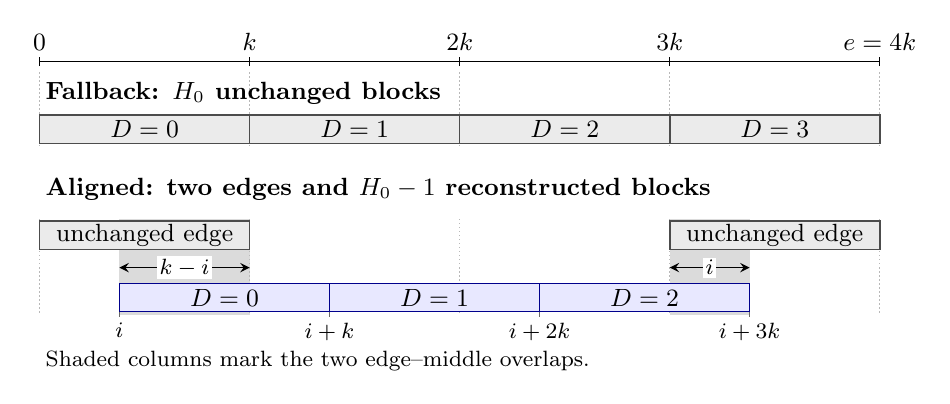
\begin{tikzpicture}[
    x=.22\linewidth,y=8mm,
    font=\small,
    every node/.style={inner sep=2pt},
    original/.style={draw=black!70,fill=black!8,line width=.55pt},
    reconstructed/.style={draw=blue!55!black,fill=blue!9,line width=.55pt},
    overlap/.style={fill=black!14,draw=none},
    guide/.style={draw=black!28,densely dotted,line width=.45pt}
  ]
    \def\blockoffset{.38}

    \draw[line width=.55pt] (0,5.15) -- (4,5.15);
    \foreach \x/\lab in {0/0,1/k,2/2k,3/3k,4/{e=4k}} {
      \draw (\x,5.08) -- (\x,5.22);
      \node[above] at (\x,5.23) {$\lab$};
      \draw[guide] (\x,4.98) -- (\x,3.78);
    }

    \node[anchor=west,font=\small\bfseries] at (0,4.65)
      {Fallback: $H_0$ unchanged blocks};
    \foreach \D in {0,1,2,3} {
      \draw[original] (\D,3.85) rectangle ({\D+1},4.30);
      \node at ({\D+.5},4.075) {$D=\D$};
    }

    \node[anchor=west,font=\small\bfseries] at (0,3.12)
      {Aligned: two edges and $H_0-1$ reconstructed blocks};

    \path[overlap] (\blockoffset,1.13) rectangle (1,2.65);
    \path[overlap] (3,1.13) rectangle ({3+\blockoffset},2.65);
    \foreach \x in {0,1,2,3,4} {
      \draw[guide] (\x,2.65) -- (\x,1.13);
    }
    \draw[original] (0,2.17) rectangle (1,2.62);
    \draw[original] (3,2.17) rectangle (4,2.62);
    \node at (.5,2.395) {unchanged edge};
    \node at (3.5,2.395) {unchanged edge};

    \foreach \D in {0,1,2} {
      \draw[reconstructed]
        ({\blockoffset+\D},1.18)
        rectangle ({\blockoffset+\D+1},1.63);
      \node at ({\blockoffset+\D+.5},1.405) {$D=\D$};
    }
    \foreach \D/\lab in {0/i,1/{i+k},2/{i+2k},3/{i+3k}} {
      \draw[black!60] ({\blockoffset+\D},1.10)
        -- ({\blockoffset+\D},1.18);
      \node[below,font=\footnotesize] at ({\blockoffset+\D},1.10)
        {$\lab$};
    }

    \draw[<->,>=stealth,line width=.5pt]
      (\blockoffset,1.88) -- (1,1.88)
      node[midway,font=\footnotesize,fill=white,inner sep=1pt] {$k-i$};
    \draw[<->,>=stealth,line width=.5pt]
      (3,1.88) -- ({3+\blockoffset},1.88)
      node[midway,font=\footnotesize,fill=white,inner sep=1pt] {$i$};
    \node[anchor=west,font=\footnotesize] at (0,.40)
      {Shaded columns mark the two edge--middle overlaps.};
  \end{tikzpicture}
  \endgroup
  \caption{Aligned and fallback coverage of one macro-interval, translated
    to $[0,e)$. The schematic uses $H_0=4$ and $0<i<k$; every bar denotes
    a half-open interval of length $k$. In general, $e=kH_0$, and the
    middle blocks, with starts $i+Dk$ for $0\le D<H_0-1$, cover
    $[i,e-k+i)$. The unchanged edges $[0,k)$ and $[e-k,e)$ complete the
    coverage. Their overlaps with the middle union are $[i,k)$ and
    $[e-k,e-k+i)$, of lengths $k-i$ and $i$. All blocks lie in $[0,e)$.
    The fallback blocks partition $[0,e)$; at $i=0$, the first middle
    block duplicates the left edge.}
  \label{fig:block-allocation}
\end{figure}


Doing this in all $uJ$ macro-intervals shows that the whole
preimage of the chosen target open set is contained in one
fixed member of $\mathcal U^{[0,uN)}$.  The assertion is about
the whole preimage; no injectivity of $\Phi_u$ is required.

\paragraph{A finite subcomplex of smaller dimension.}
The target description now retains every member of the orbit-cover
information. It remains to bound the dimension of a single subcomplex
containing its image; this is where the pointwise boundary count produces
the strict decrease in cover rate.
Equip the products of copies of $S$ with their product cells,
the joins with the joins of those cells and their endpoint
cells, and $\mathcal K_u$ with the resulting product cell
structure.  These are finite polytopal complexes and admit
compatible simplicial subdivisions.  In a join, the carrier
dimension is the dimension of the retained branch at an
endpoint and is the sum of the two carrier dimensions plus
one when both weights are positive.  Product carrier
dimensions add.

Call a macro-interval good at $x$ if $w(h^{T_{b,q}}x)=1$,
and bad otherwise.  Apply \Cref{eq:cover-macro-frequency}
to $y=h^{bN}x$ in each of the $u$ windows.  The number
$B_u(x)$ of bad macro-intervals satisfies
\begin{equation}
\label{eq:cover-bad-count}
 B_u(x)\le b_0uJ.
\end{equation}
Each macro-interval has $(H_0-1)g$ replacement slots.
Consequently at most $b_0un$ of the boundary slots in
\Cref{eq:cover-total-successes} can belong to bad intervals.
If $S_u^{\mathrm{good}}(x)$ is the number of boundary slots
in good intervals, then
\begin{equation}
\label{eq:cover-good-successes}
 S_u^{\mathrm{good}}(x)\ge(a/8-b_0)un.
\end{equation}

At a good interval the join is at its aligned endpoint.
The two unchanged edge factors cost at most $2m$, and
\Cref{eq:cover-updated-carrier} bounds the other factors.
Thus its carrier dimension is at most
\[
 (H_0+1)m-\sum_{D=0}^{H_0-2}s_{b,q,D}(x).
\]
At a bad interval we may ignore all successful slots.  Its
carrier dimension is at most $(2H_0+1)m+1$: this bounds
the sum of the aligned and fallback dimensions plus one,
and also bounds the fallback endpoint.  Using
\Cref{eq:cover-bad-count,eq:cover-good-successes},
the carrier dimension of $\Phi_u(x)$ is therefore at most
\begin{align*}
 &(uJ-B_u(x))(H_0+1)m
   +B_u(x)((2H_0+1)m+1)-S_u^{\mathrm{good}}(x)\\
 &\qquad\le uJ\bigl((H_0+1)m+b_0(H_0m+1)\bigr)
                 -(a/8-b_0)un\\
 &\qquad= uJ\bigl((H_0+1)m+b_0(H_0m+1)
                   -(a/8-b_0)(H_0-1)g\bigr)
   =uNE_k.
\end{align*}
It follows that $\Phi_u(X)$ lies in the finite subcomplex
consisting of all cells of dimension at most
$\lfloor uNE_k\rfloor$, together with their faces.  In
particular this is an actual subcomplex dimension bound,
not a bound on dimensions of fibers or on a varying family
of images.

Restrict the finite target open cover constructed above
to this subcomplex, triangulate it compatibly, and apply
\Cref{lem:polyhedral-refinement}.  We obtain
\[
 D(\mathcal U^{[0,uN)})\le\lfloor uNE_k\rfloor,
 \qquad
 \frac{D(\mathcal U^{[0,uN)})}{uN}\le E_k<d.
\]
By \Cref{eq:finite-cover-rate}, $d$ is the infimum of all normalized
cover orders, so even one such $u$ gives a contradiction.  This proves
the theorem.
\end{proof}

\subsection{The extended-real equality}

\begin{proof}[Proof of \Cref{thm:main}]
Put $A=C(X)\rtimes_h\Z$.
Minimality and infinitude imply that $h$ is free: a periodic
orbit would be a finite nonempty closed invariant subset of
$X$, and hence all of $X$.  Niu's upper bound therefore gives
\begin{equation}
\label{eq:final-niu-upper-bound}
 \rc(C(X)\rtimes_h\Z)\le\frac12\mdim(X,h)
\end{equation}
in the extended nonnegative reals
\cite[Theorem~5.6]{Niu2024}.

Let $\mathcal R$ be the set of finite comparison bounds in
the definition of the radius of comparison.  For every
$r\in\mathcal R$, \Cref{thm:cover-bound} and the supremum
over all finite open covers give
\[
 \mdim(X,h)\le2r.
\]
If $\mathcal R$ is nonempty, taking its infimum yields
$\mdim(X,h)/2\le\rc(A)$.  This passage does not require
the infimum itself to belong to $\mathcal R$.  If
$\mathcal R$ is empty, the same lower inequality holds
because $\rc(A)=\infty$ by definition.  Together with
\Cref{eq:final-niu-upper-bound}, this proves the equality.

Explicitly, when $\mdim(X,h)=\infty$,
\Cref{thm:cover-bound} excludes every finite comparison
bound, so $\rc(A)=\infty$.  When $\mdim(X,h)=0$,
\Cref{eq:final-niu-upper-bound} and nonnegativity give
$\rc(A)=0$.  The argument above covers all intervening
finite values with the same trace normalization.
\end{proof}

\section{Zero mean dimension and regularity}
\label{sec:regularity-proof}

We now prove the characterization stated in \Cref{cor:regularity}.
The new equality supplies the implication from crossed-product
regularity back to zero mean dimension; the other directions use the
established results identified in the introduction.

\begin{proof}[Proof of \Cref{cor:regularity}]
Write $A=C(X)\rtimes_h\Z$ as in the corollary. This crossed product
is simple and nuclear
\cite[Section~3]{ElliottNiu2017}. It is also separable and unital, since
\(C(X)\) is separable and unital and the acting group is countable.
The canonical inclusion \(C(X)\subset A\) makes \(A\)
infinite-dimensional because \(X\) is infinite.

Lindenstrauss--Weiss proved that the small boundary property implies
zero mean dimension \cite[Theorem~5.4]{LindenstraussWeiss2000}.
Lindenstrauss proved the reverse implication for systems with an infinite
minimal factor \cite[Theorem~6.2]{Lindenstrauss1999}; here the identity
map supplies that factor. These directions are also recalled together
in \cite[Theorem~2.3]{ElliottNiu2017}. Elliott--Niu's Theorem~4.7 gives
Jiang--Su stability from zero mean dimension.

For the converse, suppose that \(A\) is Jiang--Su stable. Take
\(a,b\in M_\infty(A)_+\) with \(d_\tau(a)<d_\tau(b)\) for every
normalized trace \(\tau\) on \(A\), and place both elements in a common
finite corner \(M_q(A)\). This algebra is simple, exact, unital and
Jiang--Su stable. Every normalized trace on \(M_q(A)\) is
\(\tau\otimes\operatorname{tr}_q\) for a normalized trace \(\tau\) on
\(A\), where \(\operatorname{tr}_q=\operatorname{Tr}_q/q\). Thus, for
\(c\in M_q(A)_+\), its rank function for that normalized matrix trace is
\[
\lim_{m\to\infty}(\tau\otimes\operatorname{tr}_q)(c^{1/m})
   =\frac1q d_\tau(c),
\]
where the right side uses the unnormalized matrix extension fixed in
\Cref{eq:comparison-bound}. The strict rank inequalities therefore
hold for every normalized trace on \(M_q(A)\). R\o rdam's comparison
theorem \cite[Corollary~4.6]{Rordam2004} gives
\(a\precsim_{M_q(A)}b\), hence \(a\precsim b\) in the convention of this
paper. Thus \(0\) itself is a comparison bound, so \(\rc(A)=0\), and
\Cref{thm:main} gives
\(\mdim(X,h)=0\).

Finally, the crossed product satisfies all the hypotheses of
\cite[Theorems~A and~B]{CastillejosEvingtonTikuisisWhiteWinter2021}:
it is simple, separable, unital, nuclear and infinite-dimensional.
Finite nuclear dimension implies Jiang--Su stability by Winter's theorem
\cite{Winter2012}; the converse, with nuclear dimension at most one,
is supplied by Castillejos--Evington--Tikuisis--White--Winter.
Thus Jiang--Su stability, finite nuclear dimension and nuclear dimension
at most one are equivalent for $A$. This proves the five equivalences.
If $\mdim(X,h)>0$, including the value $\infty$, their contrapositives
give the final assertion.
\end{proof}


\begingroup
\raggedright
\bibliographystyle{plain}
\bibliography{references}
\endgroup
\end{document}
